This Chapter presents all the experiments performed and the achieved results.
Firstly, some theoretical aspects of each experimental phase are introduced, then all the experiments are clearly illustrated to make them reproducible and the obtained results are explained.

All the CPU experiments have been conducted using an Intel Core i9, with 8 cores and a frequency of 2,3 GHz.
On the other hand, the synthesis experiments utilized an AMD Virtex UltraScale+ (Alveo U280) FPGA\@.

\section{Model analysis and profiling}
\label{sec:model-analysis}%

\begin{table}[b]
\centering
    \begin{tabular}{|p{6em} c c c c|}
    \hline
%    \rowcolor{black!40}
    \textbf{Name} & \textbf{Self CPU \%} & \textbf{Self CPU} & \textbf{CPU total \%} & \textbf{CPU total} \T\B \\
    \hline \hline
    \textbf{aten::mm} & 50,25\% & 1,012$ms$ & 89,72\% & 1,807$ms$ \T\B\\
    \hline
    \textbf{aten::addmm} & 36,30\% & 731,0$\mu s$ & 37,04\% & 746,0$\mu s$ \T\B\\
    \hline
    \textbf{aten::add} & 4,67\% & 94,0$\mu s$ & 4,67\% & 94,0$\mu s$ \T\B\\
    \hline
    %\textbf{aten::\_log\_softmax} & 2,98\% & 60,0us & 2,98\% & 60,0us \T\B\\
    %\hline
    \end{tabular}
    \\[10pt]
    \caption{Excerpt of GCN model inference profiling result}
    \label{tab:gcn_profiling}
\end{table}

As already anticipated in Section~\ref{sec:toolchain-pytorch}, the GCN model, whose class is shown in Listing~\ref{lst:gcn-class}, is implemented in PyTorch, and it is characterized by two convolutional layers, a ReLU and a dropout functions.
The forward function of each layer, shown in Listing~\ref{lst:gcn-layer-forward}, is characterized by two matrix multiplications, and one of the two is a sparse multiplication.

The first step to understanding how to accelerate the PyTorch GCN model used was to analyze and profile it.
Table~\ref{tab:gcn_profiling} shows the results of one result of the profiling done using the PyTorch profiler.

The distinction between \textit{self CPU time} and \textit{total CPU time} lies in the fact that self CPU time does not contain the time spent in child operator calls, whereas total CPU time contains it, considering that operators can invoke other operators.
It is clear that the bottleneck and the most time-consuming operation is the matrix multiplication.
In particular, more than 50\% of the self CPU time is used by matrix multiplication, while, considering the child operator calls, this percentage represents nearly the 90\%.
This result clearly justifies the part of this research dedicated to matrix multiplication acceleration.

\begin{lstlisting}[language=Python,label={lst:gcn-class}, numbers=left, xleftmargin=2em, caption=Class of GCN model]
import torch.nn as nn
import torch.nn.functional as F
from pygcn.layers import GraphConvolution

class GCN(nn.Module):
    def __init__(self, nfeat, nhid, nclass, dropout):
        super(GCN, self).__init__()

        self.gc1 = GraphConvolution(nfeat, nhid)
        self.gc1 = GraphConvolution(nhid, nclass)
        self.dropout = dropout

    def forward(self, x, adj):
        x = F.relu(self.gc1(x, adj))
        x = F.dropout(x, self.dropout,
                      training=self.training)
        x = self.gc2(x, adj)
        return F.log_softmax(x, dim=1)
\end{lstlisting}


\begin{lstlisting}[language=Python,label={lst:gcn-layer-forward}, numbers=left, xleftmargin=2em, caption=Forward function of GCN layer]
    def forward(self, input, adj):
        support = torch.mm(input, self.weight)
        output = torch.spmm(adj, support)
        if self.bias is not None:
            return output + self.bias
        else:
            return output
\end{lstlisting}

\section{Matrix multiplication acceleration}
\label{sec:matmul-acceleration}%

Matrix multiplication is a well-known algorithm.
It consists of multiplying two compatible matrices to obtain the result matrix.
A lot of work has been done to try to improve its performance on different architectures~\cite{DBLP:journals/corr/abs-2003-00532, opt_cuda_matmul}.

The naive implementation of the row-by-column multiplication, whose pseudocode is shown below, is characterized by three nested loops.
The multiplication is possible only in the case the number of column of the first matrix is equal to the number of row of the second one.

\begin{algorithm}[H]
    \label{alg:matmul_pseudo}
    \caption{Naive matrix multiplication algorithm}
    \label{alg:var}
    \label{protocol1}
    \begin{algorithmic}[1]
    \STATE \textbf{Data:} $A[R][P], B[M][N]$
    \STATE \textbf{Result:} $C[R][N]$
    \IF{$P == M$}
    \FOR{$m=0; m<R, m++$}
    \FOR{$r=0; r<N, r++$}
    \STATE $C[m][r] = 0$
    \FOR{$k=0; k<M, k++$}
    \STATE $C[m][r] += A[m][k] * B[k][r]$
    \ENDFOR
    \ENDFOR
    \ENDFOR
    \ENDIF
    \end{algorithmic}
\end{algorithm}

\begin{figure}[t]
    \centering
    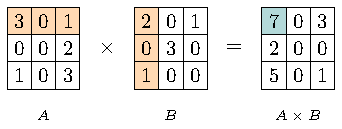
\includegraphics[height=0.24\textwidth]{Images/row-by-col-mult-example}
    \caption{Row-by-column matrix multiplication example}
    \label{fig:row-by-col-mul-example}
\end{figure}

Figure~\ref{fig:row-by-col-mul-example} highlight how an element of the output matrix is computed, using a row of the first matrix and a column of the second one.
The number of operations needed to compute a new matrix is an important parameter to try to accelerate such operation.
A calculus of this number preceded each experiments, to compute an approximation of the number of cycles needed by the accelerator.
In a general matrix multiplication, shown in the following, each element of the new matrix can be computed accordingly to Equation~\ref{eq:matmul-element}.

\[ \begin{bmatrix}
     a_{11} & a_{12} & \cdots & a_{1n}\\
     a_{21} & a_{22} & \cdots & a_{2n}\\
     \vdots & \vdots & \ddots & \vdots\\
     a_{m1} & a_{m2} & \cdots & a_{mn}
 \end{bmatrix}
 \times
 \begin{bmatrix}
     b_{11} & b_{12} & \cdots & b_{1p}\\
     b_{21} & b_{22} & \cdots & b_{2p}\\
     \vdots & \vdots & \ddots & \vdots\\
     b_{n1} & b_{n2} & \cdots & b_{np}
 \end{bmatrix}
  =
 \begin{bmatrix}
     c_{11} & c_{12} & \cdots & c_{1p}\\
     c_{21} & c_{22} & \cdots & c_{2p}\\
     \vdots & \vdots & \ddots & \vdots\\
     c_{m1} & c_{m2} & \cdots & c_{mp}
 \end{bmatrix} \]

\begin{equation}
    \label{eq:matmul-element}
    c_{ij}= a_{i1} b_{1j} + a_{i2} b_{2j} +\cdots+ a_{in} b_{nj} = \sum_{k=1}^n a_{ik}b_{kj}
\end{equation}

Then, the number of cycles needed can be calculated using Equation~\ref{eq:number-cycles}.
The first part of the Equation computes the number of cycles for the mul and add operations, while the second half computes the number of cycles needed to load and store data.
The number of cycles of the second half are computed by adding one cycle for each $ch$ operands read, and one cycle for each $ch$ operand written, with $ch$ equal to the number of memory channels.
From Listing~\ref{lst:affine-mul}, can be seen that there are three load and one store, for a total of four.

\begin{equation}
    \label{eq:number-cycles}
    cycles = (m \cdot p) \cdot ( n\cdot cycles_{mul} + (n-1) \cdot cycles_{add}) + 4 \cdot \frac{n \cdot p \cdot m}{ch}
\end{equation}

\subsection{PyTorch matrix multiplication benchmark}
\label{subsec:pytorch-matmul-bench}%

PyTorch provides different matrix representations and different matrix multiplication functions.
The one considered in this Subsection are \textit{torch.mm} and \textit{torch.spmm}.
The former function multiplies two dense matrices, but it also supports COO representation.
The latter, instead, is typically used for sparse matrix multiplications, in which one of the two matrices, or both, are saved using sparse representations.

Figure~\ref{fig:torch-mm_benchmark} represents a benchmark for the dense matrix multiplication between a first matrix of size $15 \times 15$ and a second matrix of size $15 \times 16$, both composed by float32 elements.
In particular, the plot shows five measurements computed as the average of five different executions' number.
Additionally, this average has been computed five times, and the red bar shows the range between the minimum and the maximum execution time of these repetitions.

As expected, given the high amount of executions, the five average execution times are similar between them, and the red range bar decreases as the number of executions increases.
In conclusion, the time needed by a dense matrix multiplication between two matrices of the given size is equal to 1.608$\mu s$.
The Python timing of the accelerated functions for each experiment has been computed using an average of ten millions executions.

\begin{figure}[t]
    \centering
    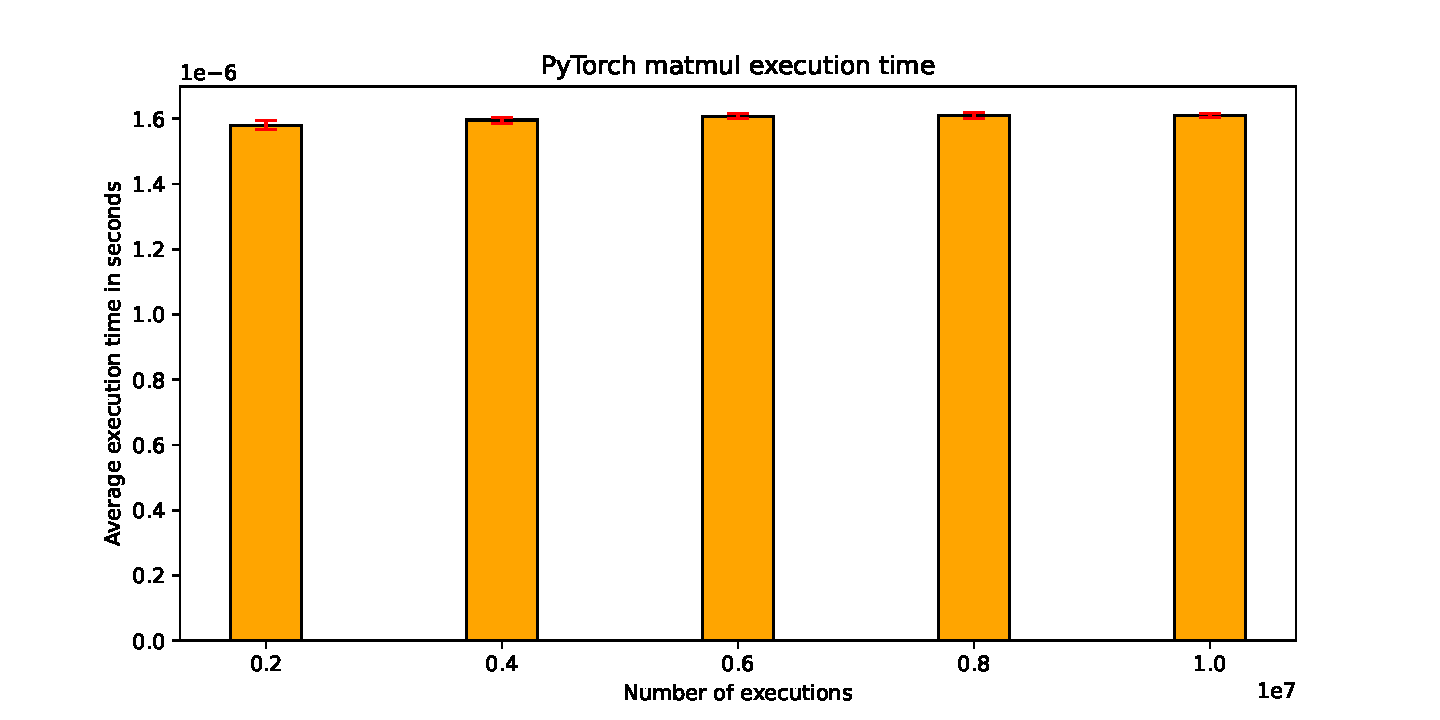
\includegraphics[height=0.4\textwidth]{Images/torch-mm_benchmark}
    \caption{Benchmark of \textit{torch.mm} PyTorch function}
    \label{fig:torch-mm_benchmark}
\end{figure}

Since the GCN model uses both dense and sparse matrix multiplication functions, Table~\ref{tab:torch-matmul-comparison} shows the times needed by both functions according to different representations of the two input matrices A and B\@.
All the times have been computed by averaging ten millions executions, the two matrices are both of size $20 \times 20$ and randomly generated; they are both composed by float32 elements and COO matrices have a sparsity of 90\%.

\begin{table}[t]
\centering
    \begin{tabular}{|p{6em} c c c |}
    \hline
    \textbf{Name} & \textbf{A, B: dense} & \textbf{A: COO, B: dense} & \textbf{A, B: COO} \T\B \\
    \hline \hline
    \textbf{torch.mm} & 1,840$\mu s$  & 3,299$\mu s$ & 16,855$\mu s$ \T\B\\
    \hline
    \textbf{torch.spmm} & 1,875$\mu s$  & 3,234$\mu s$ & 15,215$\mu s$ \T\B\\
    \hline
    \end{tabular}
    \\[10pt]
    \caption{Comparison between dense and sparse PyTorch matmul functions}
    \label{tab:torch-matmul-comparison}
\end{table}

It is clear that sparse matrix multiplication, both with dense and sparse matrix representations, does not increase performance on CPU architecture.
The advantage of using dense matrix multiplication on CPU becomes more and more evident increasing the size of the input matrices.

\subsection{Optimization comparison}
\label{subsec:optimization-comparison}%


